\section{Scalable Frequent-itemset Mining Methods}

\begin{frame}{The Downward-closure Property}

	\begin{block}{The Downward-closure Property}
		Any subset of a frequent itemset must also be frequent.
	\end{block}

	\begin{itemize}
		\item \textbf{Example:}

		      \begin{itemize}
			      \item If $\{\text{Beer, Diapers, Nuts}\}$ is frequent, so is $\{\text{Beer, Diapers}\}$.
			      \item I.e. every transaction having $\{\text{Beer, Diapers, Nuts}\}$ also contains $\{\text{Beer, Diapers}\}$.
		      \end{itemize}
		\item \textbf{Utilized by the major frequent-itemset mining algorithms:}
		      \begin{itemize}
			      \item Apriori\footnote{\fullcite{agarwal1994}}
			      \item Frequent-pattern growth (FP-growth)\footnote{\fullcite{han2000}}
			      \item etc \ldots
		      \end{itemize}
	\end{itemize}
\end{frame}

\subsection{Apriori}

\begin{frame}{Apriori Algorithm}
	\begin{block}{The Apriori Pruning Principle\footnote{\fullcite{agarwal1994}}\footnote{\fullcite{mannila1994}}}
		If there is any itemset which is infrequent, its supersets should not be generated/tested!
	\end{block}

	\begin{itemize}
		\item \textbf{The Apriori Algorithm - A Candidate Generation Approach:\footnote{A complete pseudo-code can be found in the appendix.}}
		      \begin{itemize}
			      \item Initially, scan DB once to get frequent $1$-itemsets.
			      \item Generate length-$(k+1)$ candidate itemsets from length-$k$
			            frequent itemsets.
			      \item Test the candidates against DB, discard those that are
			            infrequent.
			      \item Terminate when no further candidate or frequent itemset can
			            be generated.
		      \end{itemize}
	\end{itemize}
\end{frame}

\begin{frame}{Apriori Algorithm - Example}
	\centering
	\vspace{0cm}
	\scalebox{0.9}{%
		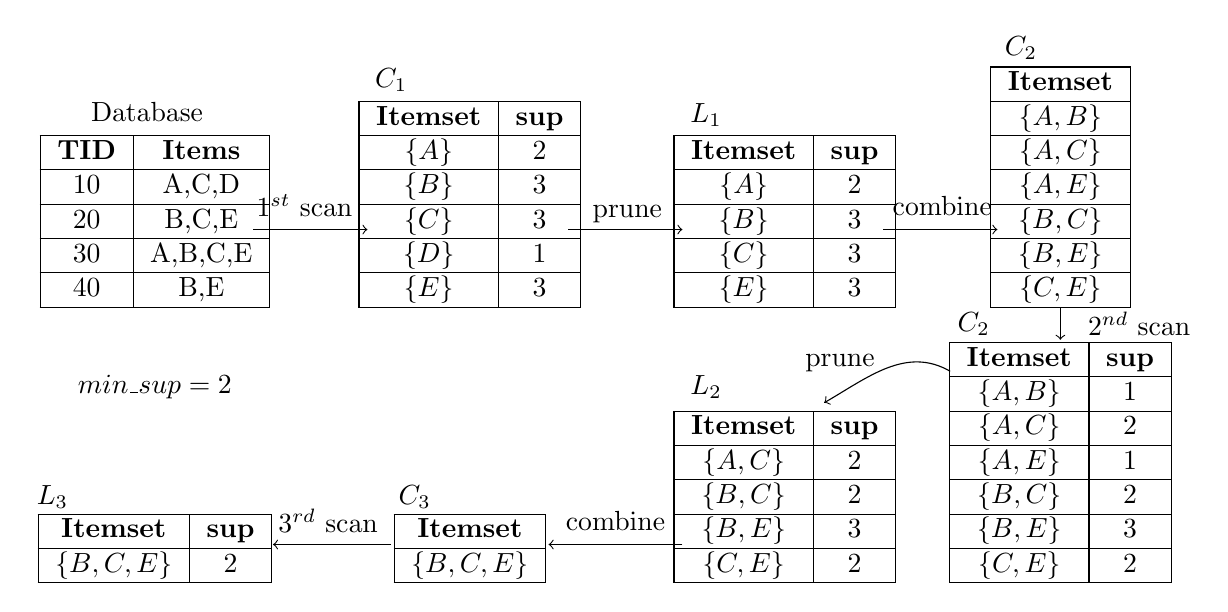
\begin{tikzpicture}
			\visible<1->{
				\path (0,1) coordinate (A) node[above, inner sep=0] {
						\begin{tabular}{ | c | c |}
							\hline
							\textbf{TID} & \textbf{Items} \\\hline
							10           & A,C,D          \\\hline
							20           & B,C,E          \\\hline
							30           & A,B,C,E        \\\hline
							40           & B,E            \\\hline
						\end{tabular}
					};
			}

			\visible<2->{
				\path (4,1) coordinate (A) node[above, inner sep=0] {
						\begin{tabular}{ | c | c |}
							\hline
							\textbf{Itemset} & \textbf{sup} \\\hline
							$\{A\}$          & 2            \\\hline
							$\{B\}$          & 3            \\\hline
							$\{C\}$          & 3            \\\hline
							$\{D\}$          & 1            \\\hline
							$\{E\}$          & 3            \\\hline
						\end{tabular}
					};
			}

			\visible<3->{
				\path (8,1) coordinate (A) node[above, inner sep=0] {
						\begin{tabular}{ | c | c |}
							\hline
							\textbf{Itemset} & \textbf{sup} \\\hline
							$\{A\}$          & 2            \\\hline
							$\{B\}$          & 3            \\\hline
							$\{C\}$          & 3            \\\hline
							$\{E\}$          & 3            \\\hline
						\end{tabular}
					};
			}

			\visible<4->{
				\path (11.5,1) coordinate (A) node[above, inner sep=0] {
						\begin{tabular}{ | c |}
							\hline
							\textbf{Itemset} \\\hline
							$\{A,B\}$        \\\hline
							$\{A,C\}$        \\\hline
							$\{A,E\}$        \\\hline
							$\{B,C\}$        \\\hline
							$\{B,E\}$        \\\hline
							$\{C,E\}$        \\\hline
						\end{tabular}
					};
			}

			\visible<5->{
				\path (11.5,-2.5) coordinate (A) node[above, inner sep=0] {
						\begin{tabular}{ | c | c |}
							\hline
							\textbf{Itemset} & \textbf{sup} \\\hline
							$\{A,B\}$        & 1            \\\hline
							$\{A,C\}$        & 2            \\\hline
							$\{A,E\}$        & 1            \\\hline
							$\{B,C\}$        & 2            \\\hline
							$\{B,E\}$        & 3            \\\hline
							$\{C,E\}$        & 2            \\\hline
						\end{tabular}
					};
			}

			\visible<6->{
				\path (8,-2.5) coordinate (A) node[above, inner sep=0] {
						\begin{tabular}{ | c | c |}
							\hline
							\textbf{Itemset} & \textbf{sup} \\\hline
							$\{A,C\}$        & 2            \\\hline
							$\{B,C\}$        & 2            \\\hline
							$\{B,E\}$        & 3            \\\hline
							$\{C,E\}$        & 2            \\\hline
						\end{tabular}
					};
			}

			\visible<7->{
				\path (4,-2.5) coordinate (A) node[above, inner sep=0] {
						\begin{tabular}{ | c |}
							\hline
							\textbf{Itemset} \\\hline
							$\{B,C,E\}$      \\\hline
						\end{tabular}
					};
			}

			\visible<8->{
				\path (0,-2.5) coordinate (A) node[above, inner sep=0] {
						\begin{tabular}{ | c | c |}
							\hline
							\textbf{Itemset} & \textbf{sup} \\\hline
							$\{B,C,E\}$      & 2            \\\hline
						\end{tabular}
					};
			}


			\visible<2->{
				\draw[->] (1.25,2) -- (2.7,2);
			}

			\visible<3->{
				\draw[->] (5.25,2) -- (6.7,2);
			}

			\visible<4->{
				\draw[->] (9.25,2) -- (10.7,2);
			}

			\visible<5->{
				\draw[->] (11.5,1) -- (11.5,0.6);
			}

			\visible<6->{
				\draw[->] (10.1,0.2) to [out=150,in=30] (8.5,-0.2);
			}

			\visible<7->{
				\draw[->] (6.7,-2) -- (5,-2);
			}

			\visible<8->{
				\draw[->] (3,-2) -- (1.5,-2);
			}


			\visible<1->{
				\node at (-0.1,3.5) {Database};
				\node at (0,0) {$min\_sup = 2$};
			}

			\visible<2->{
				\node at (1.9,2.3) {$1^{\text{st}}$ scan};
				\node at (3,3.9) {$C_1$};
			}

			\visible<3->{
				\node at (6,2.2) {prune};
				\node at (7,3.45) {$L_1$};
			}

			\visible<4->{
				\node at (10,2.3) {combine};
				\node at (11,4.3) {$C_2$};
			}

			\visible<5->{
				\node at (12.5,0.8) {$2^{\text{nd}}$ scan};
				\node at (10.4,0.8) {$C_2$};
			}

			\visible<6->{
				\node at (8.7,0.3) {prune};
				\node at (7,0) {$L_2$};
			}

			\visible<7->{
				\node at (3.3,-1.4) {$C_3$};
				\node at (5.85,-1.7) {combine};
			}

			\visible<8->{
				\node at (2.2,-1.7) {$3^{\text{rd}}$ scan};
				\node at (-1.3,-1.4) {$L_3$};
			}
		\end{tikzpicture}
	}
\end{frame}


\begin{frame}{Apriori Algorithm - Candidate Generation}
	\begin{alertblock}{Follow the Apriori Pruning Principle!}
		If \textbf{any} subset of an itemset you wish to generate is infrequent, it is \textbf{not} a valid candidate!
	\end{alertblock}

	\vspace{0.25cm}

	\begin{itemize}
		\item \textbf{Example}\footnote{Based on the previous slide/example}\textbf{:}
		      \begin{itemize}
			      \item The itemset $\{A,B,C\}$ is \textbf{not} a valid candidate:
			            \begin{itemize}
				            \item Frequent Subsets: $\{A\}$, $\{B\}$, $\{C\}$, $\{A,C\}$, $\{B,C\}$
				            \item Infrequent Subset: $\{A,B\}$
			            \end{itemize}
		      \end{itemize}
		\item \textbf{\color{airforceblue}How to generate candidates?}
		      \begin{itemize}
			      \item Step 1: Join all frequent $k$-itemsets that have $k-1$ items in
			            common.
			            \begin{itemize}
				            \item E.g. $\{A,B\}$ and $\{A,C\}$ can be joined to form $\{A,B,C\}$.
			            \end{itemize}
			      \item Step 2: Prune all combinations that have infrequent subsets.
			            \begin{itemize}
				            \item E.g. $\{A,B,C\}$ has to be pruned, because $\{A,B\}$ is infrequent.
			            \end{itemize}
		      \end{itemize}
	\end{itemize}
\end{frame}

\begin{frame}{Improvements}
	\begin{itemize}
		\item \textbf{Apriori is pretty inefficient:}
		      \begin{itemize}
			      \item Multiple scans of transaction database.
			      \item Huge number of candidates.
			      \item Support counting for candidates is laborious.
		      \end{itemize}
		\item \textbf{Many improvements have been proposed.}
		\item \textbf{Some examples:}
		      \begin{itemize}
			      \item Reducing the passes of database scans:
			            \begin{itemize}
				            \item Partitioning\footnote{e.g. \fullcite{savasere1995}}
				            \item Dynamic itemset counting\footnote{e.g. \fullcite{brin1997}}
			            \end{itemize}
			      \item Shrinking the number of candidates:
			            \begin{itemize}
				            \item Hashing\footnote{e.g. \fullcite{park1995}}
			            \end{itemize}
		      \end{itemize}
	\end{itemize}
\end{frame}

\begin{frame}{Improvements - Partitioning}
	\begin{block}{Partitioning: The Basic Idea}
		Any itemset that is potentially frequent in the whole database must be frequent in at least one of the partitions of the database.
	\end{block}
	\begin{itemize}
		\item \textbf{Method: Scan the database twice}
		      \begin{itemize}
			      \item Scan 1: Partition database and find the local frequent itemsets:
			            \begin{itemize}
				            \item $\text{min\_sup}_i = \text{min\_sup}[\%] \cdot \vert
					                  \sigma\text{DB}_i \vert$.
			            \end{itemize}
			      \item Scan 2: Use the local frequent itemsets to check for global frequent itemsets:
			            \begin{itemize}
				            \item Only itemsets that are frequent in at least one partition are checked.
			            \end{itemize}
		      \end{itemize}
	\end{itemize}
	\vspace{0.25cm}
	\centering
	\begin{tikzpicture}[square/.style={regular polygon,regular polygon sides=4}]
		\node at (0,0) [square, draw, fill=gray, minimum size=2cm] {};
		\node at (3,0) [square, draw, fill=gray, minimum size=2cm] {};
		\node at (8,0) [square, draw, fill=gray, minimum size=2cm] {};
		\node at (5.5,0) {$\hdots$};
		\node at (0,0) {DB$_1$};
		\node at (0,-1.5) {$\sup_1(i) \leq \vert\sigma \text{DB}_1\vert$};
		\node at (3,-1.5) {$\sup_2(i) \leq \vert\sigma \text{DB}_2\vert$};
		\node at (8,-1.5) {$\sup_k(i) \leq \vert\sigma \text{DB}_k\vert$};
		\node at (10.5,-0.5) {$\sup(i) \leq \vert\sigma \text{DB}\vert$};
		\node at (3,0) {DB$_2$};
		\node at (8,0) {DB$_k$};
		\node at (4.5,0) {+};
		\node at (6.5,0) {+};
		\node at (1.5,0) {+};
		\node at (10,0) {= DB};
	\end{tikzpicture}
\end{frame}

\begin{frame}{Improvements - Dynamic Itemset Counting (I)}
	\begin{block}{Dynamic Itemset Counting (DIC): The Basic Idea}
		Itemset frequency counting starts once all subsets are confirmed to be frequent.
	\end{block}

	\begin{itemize}
		\item \textbf{Candidate itemsets are added at different points during a scan:}
		      \begin{itemize}
			      \item New candidate itemsets can be added at any start point during a scan.
			            \begin{itemize}
				            \item E.g. if $A$ and $B$ are already found to be frequent, \\
				                  $AB$ are also counted from that starting point on.
			            \end{itemize}
			      \item Uses the count-so-far as the lower bound of the actual count.
			      \item If count-so-far passes minimum support, itemset is added to
			            frequent-itemset collection.
			      \item Can then be used to generate even longer candidates.
		      \end{itemize}
	\end{itemize}
\end{frame}

\begin{frame}{Improvements - Dynamic Itemset Counting (II)}
	\vspace{1cm}
	\begin{columns}
		\begin{column}{0.5\textwidth}
			\centering
			\scalebox{0.9}{
				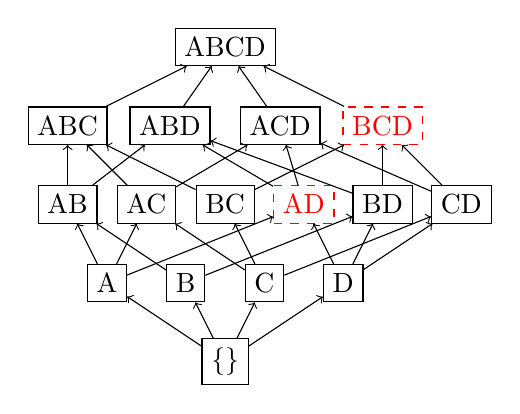
\begin{tikzpicture}
					\node[draw] at (0,0) (abcd) {ABCD};
					\node[draw] at (-2,-1) (abc) {ABC};
					\node[draw] at (-0.7,-1) (abd) {ABD};
					\node[draw] at (0.7,-1) (acd) {ACD};
					\node[draw, dashed, color=red] at (2,-1) (bcd) {BCD};

					\node[draw] at (-2,-2) (ab) {AB};
					\node[draw] at (-1,-2) (ac) {AC};
					\node[draw] at (0,-2) (bc) {BC};
					\node[draw, dashed, color=red] at (1,-2) (ad) {AD};
					\node[draw] at (2,-2) (bd) {BD};
					\node[draw] at (3,-2) (cd) {CD};

					\node[draw] at (-1.5,-3) (a) {A};
					\node[draw] at (-0.5,-3) (b) {B};
					\node[draw] at (0.5,-3) (c) {C};
					\node[draw] at (1.5,-3) (d) {D};
					\node[draw] at (0,-4) (0) {$\{\}$};

					\draw[->] (0)-- (a);
					\draw[->] (0)-- (b);
					\draw[->] (0)-- (c);
					\draw[->] (0)-- (d);
					\draw[->] (a)-- (ab);
					\draw[->] (a)-- (ac);
					\draw[->] (a)-- (ad);
					\draw[->] (b)-- (ab);
					\draw[->] (b)-- (bd);
					\draw[->] (c)-- (ac);
					\draw[->] (c)-- (bc);
					\draw[->] (c)-- (cd);
					\draw[->] (d)-- (ad);
					\draw[->] (d)-- (bd);
					\draw[->] (d)-- (cd);

					\draw[->] (ab)-- (abc);
					\draw[->] (ab)-- (abd);
					\draw[->] (ac)-- (abc);
					\draw[->] (ac)-- (acd);
					\draw[->] (bc)-- (abc);
					\draw[->] (bc)-- (bcd);
					\draw[->] (ad)-- (abd);
					\draw[->] (ad)-- (acd);
					\draw[->] (bd)-- (abd);
					\draw[->] (bd)-- (bcd);
					\draw[->] (cd)-- (acd);
					\draw[->] (cd)-- (bcd);

					\draw[->] (abc)-- (abcd);
					\draw[->] (abd)-- (abcd);
					\draw[->] (acd)-- (abcd);
					\draw[->] (bcd)-- (abcd);
				\end{tikzpicture}
			}
		\end{column}
		\begin{column}{0.5\textwidth}
			\vspace{-6.2cm}
			\scalebox{0.9}{
				\begin{tikzpicture}
					\node[draw, fill=gray, text width = 7cm]
					{\color{white}Transactions};
					\draw[->, color=airforceblue] (-3,-0.8) -- (3,-0.8);
					\draw[->, color=airforceblue] (-3,-1.3) -- (3,-1.3);
					\draw[->, color=airforceblue] (-3,-1.8) -- (3,-1.8);
					\draw[->, color=red] (-3,-2.3) -- (3,-2.3);
					\draw[color=red] (-2,-2.8) -- (3,-2.8);
					\draw[color=red] (0,-3.3) -- (3,-3.3);
					\draw[->, color=red] (-3,-3.8) -- (-1.5,-3.8);
					\draw[->, color=red] (-3,-4.3) -- (0.5,-4.3);
					\node at (0, -0.5) {\color{airforceblue}1-itemsets};
					\node at (0, -1.1) {\color{airforceblue}2-itemsets};
					\node at (0, -2.1) {\color{red}1-itemsets};
					\node at (0, -2.6) {\color{red}2-itemsets};
					\node at (0.8, -3.1) {\color{red}3-itemsets};
					\node at (0, -1.6) {\color{airforceblue}$\ldots$};
					\draw[dashed, color=red] (3,-2.8) -- (-3,-3.8);
					\draw[dashed, color=red] (3,-3.3) -- (-3,-4.3);
					\node at (-3.5, -3.1) {\color{red}DIC:};
					\node at (-3.5, -1.1) {\color{airforceblue}Apriori:};
				\end{tikzpicture}
			}
		\end{column}
	\end{columns}
\end{frame}

\begin{frame}{Improvements - Hashing}
	\begin{block}{Hashing: The Basic Idea}
		Itemsets are hashed into buckets, and during the first scan, only the occurrences of each bucket are counted.
	\end{block}

	\begin{columns}[c]
		\begin{column}{0.6\textwidth}
			\begin{itemize}
				\item \textbf{A $k$-itemset whose corresponding hashing-bucket
					      count is below the threshold cannot be frequent.}
				      \begin{itemize}
					      \item Candidates: $a,b,c,d,e$.
					      \item While scanning DB for frequent $1$-itemsets, create
					            hash entries for $2$-itemsets:
					            \begin{itemize}
						            \item $\{ab,ad,ae\}$
						            \item $\{bd,be,de\}$
						            \item $\ldots$
					            \end{itemize}
					      \item Frequent $1$-itemset: $a,b,d,e$.
					      \item $ab$ is not a candidate $2$-itemset, if the sum of
					            count of $\{ab, ad, ae\}$ is below support threshold.
				      \end{itemize}
			\end{itemize}
		\end{column}
		\begin{column}{0.3\textwidth}
			\centering
			\textbf{Hash table:}\\
			\begin{tabular}{| c | c |}
				\hline
				count    & itemsets       \\\hline
				35       & $\{ab,ad,ae\}$ \\\hline
				88       & $\{bd,be,de\}$ \\\hline
				$\vdots$ & $\vdots$       \\\hline
				102      & $\{yz,qs,wt\}$ \\\hline
			\end{tabular}
		\end{column}
	\end{columns}
\end{frame}

\subsection{FP-growth}

\begin{frame}{FP-growth}
	\begin{itemize}
		\item \textbf{Apriori:}
		      \begin{itemize}
			      \item Breadth-first (i.e., level-wise) search.
			      \item Candidate generation and test.
			            \begin{itemize}
				            \item Often generates a huge number of candidates.
			            \end{itemize}
		      \end{itemize}
		\item \textbf{FP-growth:}
		      \begin{itemize}
			      \item Depth-first search.
			      \item Avoid explicit candidate generation.
		      \end{itemize}
	\end{itemize}

	\vspace{0.5cm}

	\begin{block}{FP-growth: All Frequent Itemsets in Only Two Scans}
		FP-growth employs a tree-based structure to identify all frequent itemsets in a dataset using two scans.
	\end{block}
\end{frame}

% Commands for the FP-tree
\newcommand{\fptreerootnode}{
	\begin{tikzpicture}
		\node[draw, fill=faugraydark!75, text=white, minimum height = 0.65cm, minimum width=1cm] at (0,-1) (Label) {$\{\}$};
	\end{tikzpicture}
}

\newcommand{\fptreeuniquenode}[1]{
	\begin{tikzpicture}
		\node[draw, fill=faugraydark!75, text=white, minimum height = 0.65cm, minimum width=1cm] at (0,-1) (Label) {$#1$};
	\end{tikzpicture}
}

\newcommand{\fptreenode}[2]{
	\begin{tikzpicture}
		\node[draw, fill=white, minimum height = 0.65cm, minimum width=0.5cm] at (0,-1) (Label) {$#1$};
		\node[draw, fill=faugraydark!75, text=white, minimum height = 0.65cm, minimum width=0.5cm, right = 0cm of Label] {$#2$};
	\end{tikzpicture}
}

\newcommand{\fptreenodemarked}[2]{
	\begin{tikzpicture}
		\node[draw, fill=white, minimum height = 0.65cm, minimum width=0.5cm] at (0,-1) (Label) {$#1$};
		\node[draw, fill=faureddark!75, text=white, minimum height = 0.65cm, minimum width=0.5cm, right = 0cm of Label] {$#2$};
	\end{tikzpicture}
}

\newcommand{\fptreenodeprefix}[2]{
	\begin{tikzpicture}
		\node[draw, fill=white, minimum height = 0.65cm, minimum width=0.5cm] at (0,-1) (Label) {$#1$};
		\node[draw, fill=fauorange!75, text=white, minimum height = 0.65cm, minimum width=0.5cm, right = 0cm of Label] {$#2$};
	\end{tikzpicture}
}
\newcommand{\headertableheader}{
	\begin{tikzpicture}
		\node[draw, fill=white, minimum height = 0.65cm, minimum width=1.65cm] at (0,-1) (Item) {\textbf{Item}};
		\node[draw, fill=white, minimum height = 0.65cm, minimum width=1.65cm, right = 0cm of Item] {\textbf{Sum}};
	\end{tikzpicture}
}

\newcommand{\headertableentry}[2]{
	\begin{tikzpicture}
		\node[draw, fill=white, minimum height = 0.65cm, minimum width=1.65cm] at (0,-1) (Item) {$#1$};
		\node[draw, fill=white, minimum height = 0.65cm, minimum width=1.65cm, right = 0cm of Item] {$#2$};
	\end{tikzpicture}
}

\newcommand{\headertableentrymarked}[2]{
	\begin{tikzpicture}
		\node[draw, fill=faureddark!20, minimum height = 0.65cm, minimum width=1.65cm] at (0,-1) (Item) {$#1$};
		\node[draw, fill=faureddark!20, minimum height = 0.65cm, minimum width=1.65cm, right = 0cm of Item] {$#2$};
	\end{tikzpicture}
}


\begin{frame}{FP-growth - Algorithm}
	\begin{columns}
		\begin{column}{0.45\textwidth}
			\vspace{-6.5cm}
			\begin{itemize}
				\item \textbf{Steps of FP-growth:}
				      \begin{enumerate}
					      \visible<2->{
					      \item Find frequent $1$-itemsets (\textbf{1st scan}).
					            }
					            \visible<4->{
					      \item Put them in a frequency-descending list. \\
					            \hspace{0.25cm}$\Rightarrow$ \textbf{f-list}.
					            }
					            \visible<6->{
					      \item Perform the \textbf{2nd scan:}
					            \begin{itemize}
						            \item {\only<8,11,14,17,20>{\color{faugraydark}}Sort and filter the items in each tuple.}
						            \item {\only<9,12,15,18,21>{\color{faugraydark}}Construct the initial \textbf{FP-tree}}.\visible<22->{
							                  \\
							                  \textit{(Also comes with a \textbf{header table})}
						                  }

					            \end{itemize}
					            }
					            \visible<23->{
					      \item Start the FP-tree \textbf{recursion:}
					            \begin{enumerate}
						            \visible<24->{
						            \item Determine the \textbf{conditional pattern base} (prefix paths) for each frequent item in the header table.
						                  }
						                  \visible<32->{
						            \item Build a \textbf{conditional FP-tree} for each non-empty conditional pattern base.
						                  }
						                  \visible<36->{
						            \item Perform \textbf{4.} for each cond. FP-tree.
						                  }
					            \end{enumerate}
					            }
					            \visible<56->{
					      \item Collect the \textbf{frequent itemsets}.
					            }

				      \end{enumerate}
			\end{itemize}
		\end{column}
		\begin{column}{0.45\textwidth}
			\vspace*{-0.5cm}
			\centering
			\scalebox{0.75}{
				\begin{tikzpicture}
					\visible<1-21>{
						\visible<1-21>{
							\node[text width=5cm, anchor=north] at (0,0) (original-dataset)
							{
								\begin{center}
									\begin{tabular}{|c|c|}
										\hline
										\textbf{TID}                            & \textbf{Items bought}                                                                 \\\hline
										\only<7-9>{\cellcolor{faugray!50}}100   & \only<7-9>{\cellcolor{faugray!50}}\only<1-7>{f,a,c,d,g,i,m,p}\only<8->{f,c,a,m,p}     \\\hline
										\only<10-12>{\cellcolor{faugray!50}}200 & \only<10-12>{\cellcolor{faugray!50}}\only<1-10>{a,b,c,f,l,m}\only<11->{f,c,a,b,m}     \\\hline
										\only<13-15>{\cellcolor{faugray!50}}300 & \only<13-15>{\cellcolor{faugray!50}}\only<1-13>{b,f,h,j,o,w}\only<14->{f,b}           \\\hline
										\only<16-18>{\cellcolor{faugray!50}}400 & \only<16-18>{\cellcolor{faugray!50}}\only<1-16>{b,c,k,s,p}\only<17->{c,b,p}           \\\hline
										\only<19-21>{\cellcolor{faugray!50}}500 & \only<19-21>{\cellcolor{faugray!50}}\only<1-19>{a,f,c,e,l,p,m,n}\only<20->{f,c,a,m,p} \\\hline
									\end{tabular} \\
									\vspace{0.2cm}
									$min\_sup=3$ \\
									\visible<5->{
										\vspace{0.15cm}
										\textbf{f-list:} f-c-a-b-m-p
									}
								\end{center}
							};
						}

						\visible<3-5>{
							\node[text width=5cm, anchor=north, below=0.15cm of original-dataset] (frequent-1-itemsets)
							{
								\begin{center}
									\textbf{Frequent $1$-itemsets:} \\
									\vspace{0.2cm}
									\begin{tabular}{|c|c|}
										\hline
										\textbf{Itemset} & \textbf{Support} \\\hline
										\{f\}            & 4                \\\hline
										\{a\}            & 3                \\\hline
										\{c\}            & 4                \\\hline
										\{m\}            & 3                \\\hline
										\{p\}            & 3                \\\hline
										\{b\}            & 3                \\\hline
									\end{tabular} \\
								\end{center}

							};
						}

						\visible<3>{
							\draw[->] (original-dataset.east) to [out=0, in=-0] (frequent-1-itemsets.east);
						}

						\visible<5>{
							\draw[->] (frequent-1-itemsets.east) to [out=0, in=-0] (original-dataset.south east);
						}

						\visible<9->{
							\node[text width=5cm, anchor=north, below=0cm of original-dataset] (fp-tree)
							{
								\scalebox{0.7}{
									\begin{tikzpicture} [scale=1]
										\useasboundingbox (-4,0) rectangle (4,-5.5);

										\node at (0,0) (root) {\fptreerootnode};

										% TID 100
										\visible<9-11>{
											\node at (0,-1) (f) {\fptreenode{f}{1}};
											\node at (0,-2) (fc) {\fptreenode{c}{1}};
											\node at (0,-3) (fca) {\fptreenode{a}{1}};
											\node at (0,-4) (fcam) {\fptreenode{m}{1}};
											\node at (0,-5) (fcamp) {\fptreenode{p}{1}};

											\draw (root) -- (f) -- (fc) -- (fca) -- (fcam) -- (fcamp);
										}

										% TID 200
										\visible<12-14>{
											\node at (0,-1) (f) {\fptreenode{f}{2}};
											\node at (0,-2) (fc) {\fptreenode{c}{2}};
											\node at (0,-3) (fca) {\fptreenode{a}{2}};
											\node at (-1,-4) (fcam) {\fptreenode{m}{1}};
											\node at (-1,-5) (fcamp) {\fptreenode{p}{1}};
											\node at (1,-4) (fcab) {\fptreenode{b}{1}};
											\node at (1,-5) (fcabm) {\fptreenode{m}{1}};

											\draw (root) -- (f) -- (fc) -- (fca) -- (fcam) -- (fcamp);
											\draw (fca) -- (fcab) -- (fcabm);
										}

										% TID 300
										\visible<15-17>{
											\node at (0,-1) (f) {\fptreenode{f}{3}};
											\node at (-1,-2) (fc) {\fptreenode{c}{2}};
											\node at (-1,-3) (fca) {\fptreenode{a}{2}};
											\node at (-2,-4) (fcam) {\fptreenode{m}{1}};
											\node at (-2,-5) (fcamp) {\fptreenode{p}{1}};
											\node at (0,-4) (fcab) {\fptreenode{b}{1}};
											\node at (0,-5) (fcabm) {\fptreenode{m}{1}};
											\node at (1,-2) (fb) {\fptreenode{b}{1}};

											\draw (root) -- (f) -- (fc) -- (fca) -- (fcam) -- (fcamp);
											\draw (fca) -- (fcab) -- (fcabm);
											\draw (f) -- (fb);
										}

										% TID 400
										\visible<18-20>{
											\node at (-1.5,-1) (f) {\fptreenode{f}{3}};
											\node at (-2.5,-2) (fc) {\fptreenode{c}{2}};
											\node at (-2.5,-3) (fca) {\fptreenode{a}{2}};
											\node at (-3.5,-4) (fcam) {\fptreenode{m}{1}};
											\node at (-3.5,-5) (fcamp) {\fptreenode{p}{1}};
											\node at (-1.5,-4) (fcab) {\fptreenode{b}{1}};
											\node at (-1.5,-5) (fcabm) {\fptreenode{m}{1}};
											\node at (-0.5,-2) (fb) {\fptreenode{b}{1}};
											\node at (1.5,-1) (c) {\fptreenode{c}{1}};
											\node at (1.5,-2) (b) {\fptreenode{b}{1}};
											\node at (1.5,-3) (p) {\fptreenode{p}{1}};

											\draw (root) -- (f) -- (fc) -- (fca) -- (fcam) -- (fcamp);
											\draw (fca) -- (fcab) -- (fcabm);
											\draw (f) -- (fb);
											\draw (root) -- (c) -- (b) -- (p);
										}

										% TID 500
										\visible<21>{
											\node at (-1.5,-1) (f) {\fptreenode{f}{4}};
											\node at (-2.5,-2) (fc) {\fptreenode{c}{3}};
											\node at (-2.5,-3) (fca) {\fptreenode{a}{3}};
											\node at (-3.5,-4) (fcam) {\fptreenode{m}{2}};
											\node at (-3.5,-5) (fcamp) {\fptreenode{p}{2}};
											\node at (-1.5,-4) (fcab) {\fptreenode{b}{1}};
											\node at (-1.5,-5) (fcabm) {\fptreenode{m}{1}};
											\node at (-0.5,-2) (fb) {\fptreenode{b}{1}};
											\node at (1.5,-1) (c) {\fptreenode{c}{1}};
											\node at (1.5,-2) (b) {\fptreenode{b}{1}};
											\node at (1.5,-3) (p) {\fptreenode{p}{1}};

											\draw (root) -- (f) -- (fc) -- (fca) -- (fcam) -- (fcamp);
											\draw (fca) -- (fcab) -- (fcabm);
											\draw (f) -- (fb);
											\draw (root) -- (c) -- (b) -- (p);
										}

									\end{tikzpicture}
								}
							};
						}

						\visible<9,12,15,18,21>{
							\draw[->] (original-dataset.east) to [out=0, in=-0] (fp-tree.east);
						}

					}

					\visible<22-33,38,42,44,52>{
						% Header table
						\node[inner sep=0cm] at (-2,-1.5) (headertable) {\scalebox{0.7}{\headertableheader}};
						\node[inner sep=0cm, below=0cm of headertable]  (f-header) {\scalebox{0.7}{%
								\only<22-25,27->{%
									\headertableentry{f}{4}%
								}%
								\only<26>{%
									\headertableentrymarked{f}{4}%
								}%
							}};
						\node[inner sep=0cm, below=0cm of f-header] (c-header) {\scalebox{0.7}{%
								\only<22-26,28->{%
									\headertableentry{c}{4}%
								}%
								\only<27>{%
									\headertableentrymarked{c}{4}%
								}%
							}};
						\node[inner sep=0cm, below=0cm of c-header] (a-header) {\scalebox{0.7}{%
								\only<22-27,29->{%
									\headertableentry{a}{3}%
								}%
								\only<28>{%
									\headertableentrymarked{a}{3}%
								}%
							}};
						\node[inner sep=0cm, below=0cm of a-header] (b-header) {\scalebox{0.7}{%
								\only<22-28,30->{%
									\headertableentry{b}{3}%
								}%
								\only<29>{%
									\headertableentrymarked{b}{3}%
								}%
							}};
						\node[inner sep=0cm, below=0cm of b-header] (m-header) {\scalebox{0.7}{%
								\only<22-29,31->{%
									\headertableentry{m}{3}%
								}%
								\only<30>{%
									\headertableentrymarked{m}{3}%
								}%
							}};
						\node[inner sep=0cm, below=0cm of m-header] (p-header) {\scalebox{0.7}{%
								\only<22-30,32->{%
									\headertableentry{p}{3}%
								}%
								\only<31>{%
									\headertableentrymarked{p}{3}%
								}%
							}};

						% FP-tree
						\node[inner sep=0.05cm] at (3,-1) (root) {\scalebox{0.7}{%
								\fptreerootnode%
							}};

						% F
						\node[inner sep=0.05cm] at (1.95,-1.7) (f) {\scalebox{0.7}{%
								\only<22-25,32->{%
									\fptreenode{f}{4}%
								}%
								\only<26>{%
									\fptreenodemarked{f}{4}%
								}%
								\only<27,28,29,30,31>{%
									\fptreenodeprefix{f}{4}%
								}%
							}};

						% C
						\node[inner sep=0.05cm] at (1.25,-2.4) (fc) {\scalebox{0.7}{%
								\only<22-26,32->{%
									\fptreenode{c}{3}%
								}%
								\only<27>{%
									\fptreenodemarked{c}{3}%
								}%
								\only<28,29,30,31>{%
									\fptreenodeprefix{c}{3}%
								}%
							}};
						\node[inner sep=0.05cm] at (4.05,-1.7) (c) {\scalebox{0.7}{%
								\only<22-26,28,30,32->{%
									\fptreenode{c}{1}%
								}%
								\only<27>{%
									\fptreenodemarked{c}{1}%
								}%
								\only<29,31>{%
									\fptreenodeprefix{c}{1}%
								}%
							}};

						% A
						\node[inner sep=0.05cm] at (1.25,-3.1) (fca) {\scalebox{0.7}{%
								\only<22-27,32->{%
									\fptreenode{a}{3}%
								}%
								\only<28>{%
									\fptreenodemarked{a}{3}%
								}%
								\only<29,30,31>{%
									\fptreenodeprefix{a}{3}%
								}%
							}};

						% B
						\node[inner sep=0.05cm] at (1.95,-3.8) (fcab) {\scalebox{0.7}{%
								\only<22-28,31->{%
									\fptreenode{b}{1}%
								}%
								\only<29>{%
									\fptreenodemarked{b}{1}%
								}%
								\only<30>{%
									\fptreenodeprefix{b}{1}%
								}%
							}};
						\node[inner sep=0.05cm] at (2.65,-2.4) (fb) {\scalebox{0.7}{%
								\only<22-28,30->{%
									\fptreenode{b}{1}%
								}%
								\only<29>{%
									\fptreenodemarked{b}{1}%
								}%
							}};
						\node[inner sep=0.05cm] at (4.05,-2.4) (cb) {\scalebox{0.7}{%
								\only<22-28,30,32->{%
									\fptreenode{b}{1}%
								}%
								\only<29>{%
									\fptreenodemarked{b}{1}%
								}%
								\only<31>{%
									\fptreenodeprefix{b}{1}%
								}%
							}};

						% M
						\node[inner sep=0.05cm] at (0.55,-3.8) (fcam) {\scalebox{0.7}{%
								\only<22-29,32->{%
									\fptreenode{m}{2}%
								}%
								\only<30>{%
									\fptreenodemarked{m}{2}%
								}%
								\only<31>{%
									\fptreenodeprefix{m}{2}%
								}%
							}};
						\node[inner sep=0.05cm] at (1.95,-4.5) (fcabm) {\scalebox{0.7}{%
								\only<22-29,31->{%
									\fptreenode{m}{1}%
								}%
								\only<30>{%
									\fptreenodemarked{m}{1}%
								}%
							}};

						% P
						\node[inner sep=0.05cm] at (0.55,-4.5) (fcamp) {\scalebox{0.7}{%
								\only<22-30,32->{%
									\fptreenode{p}{2}%
								}%
								\only<31>{%
									\fptreenodemarked{p}{2}%
								}%
							}};
						\node[inner sep=0.05cm] at (4.05,-3.1) (cbp) {\scalebox{0.7}{%
								\only<22-30,32->{%
									\fptreenode{p}{1}%
								}%
								\only<31>{%
									\fptreenodemarked{p}{1}%
								}%
							}};

						% Connections
						\draw (root) -- (f) -- (fc) -- (fca) -- (fcam) -- (fcamp);
						\draw (fca) -- (fcab) -- (fcabm);
						\draw (f) -- (fb);
						\draw (root) -- (c) -- (cb) -- (cbp);

						% Pointers
						% F
						\visible<22-25,27->{
							\draw[->, color=faugraydark, dashed] (f-header) to [out=0, in=180] (f);
						}
						\visible<26>{
							\draw[->, color=faureddark, dashed] (f-header) to [out=0, in=180] (f);
						}

						% C
						\visible<22-26,28->{
							\draw[->, color=faugraydark, dashed] (c-header) to [out=0, in=180] (fc);
							\draw[->, color=faugraydark, dashed] (fc) .. controls (2.5,-2.0) and (3.5,-1.7) .. (c);
						}
						\visible<27>{
							\draw[->, color=faureddark, dashed] (c-header) to [out=0, in=180] (fc);
							\draw[->, color=faureddark, dashed] (fc) .. controls (2.5,-2.0) and (3.5,-1.7) .. (c);
						}

						% A
						\visible<22-27,29->{
							\draw[->, color=faugraydark, dashed] (a-header) to [out=0, in=180] (fca);
						}
						\visible<28>{
							\draw[->, color=faureddark, dashed] (a-header) to [out=0, in=180] (fca);
						}

						% B
						\visible<22-28,30->{
							\draw[->, color=faugraydark, dashed] (b-header) to [out=0, in=155] (fcab);
							\draw[->, color=faugraydark, dashed] (fcab) to [out=0, in=270] (fb);
							\draw[->, color=faugraydark, dashed] (fb) to [out=0, in=180] (cb);
						}
						\visible<29>{
							\draw[->, color=faureddark, dashed] (b-header) to [out=0, in=155] (fcab);
							\draw[->, color=faureddark, dashed] (fcab) to [out=0, in=270] (fb);
							\draw[->, color=faureddark, dashed] (fb) to [out=0, in=180] (cb);
						}

						% M
						\visible<22-29,31->{
							\draw[->, color=faugraydark, dashed] (m-header) to [out=0, in=180] (fcam);
							\draw[->, color=faugraydark, dashed] (fcam) to [out=0, in=180] (fcabm);
						}
						\visible<30>{
							\draw[->, color=faureddark, dashed] (m-header) to [out=0, in=180] (fcam);
							\draw[->, color=faureddark, dashed] (fcam) to [out=0, in=180] (fcabm);
						}

						% P
						\visible<22-30,32->{
							\draw[->, color=faugraydark, dashed] (p-header) to [out=0, in=180] (fcamp);
							\draw[->, color=faugraydark, dashed] (fcamp) .. controls (1.95,-5) and (3.5,-5) .. (cbp);
						}
						\visible<31>{
							\draw[->, color=faureddark, dashed] (p-header) to [out=0, in=180] (fcamp);
							\draw[->, color=faureddark, dashed] (fcamp) .. controls (1.95,-5) and (3.5,-5) .. (cbp);
						}

						% Conditional pattern bases
						\visible<25->{
							\node[text width=5cm, anchor=north] at (1,-5.5) (conditional-pattern-bases)
							{
								\begin{tabular}{|c|c|}
									\hline
									\textbf{Item}                                                          & \textbf{Conditional Pattern Base}                                                                      \\\hline
									\only<26>{\cellcolor{faureddark!20}}f                                  & \only<26>{\cellcolor{faureddark!20}}\visible<26->{-}                                                   \\\hline
									\only<27>{\cellcolor{faureddark!20}}\only<33>{\cellcolor{faugray!50}}c & \only<33>{\cellcolor{faugray!50}}\only<27>{\cellcolor{faureddark!20}}\visible<27->{f:3}                \\\hline
									\only<28>{\cellcolor{faureddark!20}}\only<38>{\cellcolor{faugray!50}}a & \only<38>{\cellcolor{faugray!50}}\only<28>{\cellcolor{faureddark!20}}\visible<28->{f,c:3}              \\\hline
									\only<29>{\cellcolor{faureddark!20}}\only<42>{\cellcolor{faugray!50}}b & \only<42>{\cellcolor{faugray!50}}\only<29>{\cellcolor{faureddark!20}}\visible<29->{f,c,a:1, f:1, c:1}  \\\hline
									\only<30>{\cellcolor{faureddark!20}}\only<44>{\cellcolor{faugray!50}}m & \only<44>{\cellcolor{faugray!50}}\only<30>{\cellcolor{faureddark!20}}\visible<30->{f,c,a:2, f,c,a,b:1} \\\hline
									\only<31>{\cellcolor{faureddark!20}}\only<52>{\cellcolor{faugray!50}}p & \only<52>{\cellcolor{faugray!50}}\only<31>{\cellcolor{faureddark!20}}\visible<31->{f,c,a,m:2, c,b:1}   \\\hline
								\end{tabular}
							};
						}
					}

					% Conditional FP-tree for "c"
					\visible<34-37>{
						\node[text width=5cm, anchor=north] at (1,0) (conditional-pattern-base)
						{
							\begin{center}
								\begin{tabular}{|c|c|}
									\hline
									\textbf{Condition} & \textbf{Pattern Base} \\\hline
									c                  & f:3                   \\\hline
								\end{tabular}
							\end{center}
						};


						\visible<35->{
							% Header table
							\node[inner sep=0cm] at (0.2,-3.1) (headertable) {\scalebox{0.7}{\headertableheader}};
							\node[inner sep=0cm, below=0cm of headertable]  (f-header) {\scalebox{0.7}{%
									\headertableentry{(c,)f}{3}%
								}};

							% FP-tree
							\node[inner sep=0.05cm] at (2.5,-3) (root) {\scalebox{0.7}{%
									\fptreerootnode%
								}};
							\node[inner sep=0.05cm] at (2.5,-3.7) (f) {\scalebox{0.7}{%
									\fptreenode{f}{3}%
								}};
							\draw (root) -- (f);


							% Pointers
							\draw[->, color=faugraydark, dashed] (f-header) to [out=0, in=180] (f);
						}

						\visible<37->{
							\node[text width=5cm, anchor=north] at (1,-5.5) (conditional-pattern-bases)
							{
								\begin{center}
									\begin{tabular}{|c|c|}
										\hline
										\textbf{Item} & \textbf{Conditional Pattern Base} \\\hline
										(c,) f        & -                                 \\\hline
									\end{tabular}
								\end{center}
							};
						}
					}


					% Conditional FP-tree for "a"
					\visible<39-40>{
						\node[text width=5cm, anchor=north] at (1,0) (conditional-pattern-base)
						{
							\begin{center}
								\begin{tabular}{|c|c|}
									\hline
									\textbf{Condition} & \textbf{Pattern Base} \\\hline
									a                  & f,c:3                 \\\hline
								\end{tabular}
							\end{center}
						};


						% Header table
						\node[inner sep=0cm] at (0.2,-3.1) (headertable) {\scalebox{0.7}{\headertableheader}};
						\node[inner sep=0cm, below=0cm of headertable]  (f-header) {\scalebox{0.7}{%
								\headertableentry{(a,)f}{3}%
							}};
						\node[inner sep=0cm, below=0cm of f-header] (c-header) {\scalebox{0.7}{%
								\headertableentry{(a,)c}{3}%
							}};

						% FP-tree
						\node[inner sep=0.05cm] at (2.5,-3) (root) {\scalebox{0.7}{%
								\fptreerootnode%
							}};
						\node[inner sep=0.05cm] at (2.5,-3.7) (f) {\scalebox{0.7}{%
								\fptreenode{f}{3}%
							}};
						\node[inner sep=0.05cm] at (2.5,-4.4) (fc) {\scalebox{0.7}{%
								\fptreenode{c}{3}%
							}};
						\draw (root) -- (f) -- (fc);


						% Pointers
						\draw[->, color=faugraydark, dashed] (f-header) to [out=0, in=180] (f);
						\draw[->, color=faugraydark, dashed] (c-header) to [out=0, in=180] (fc);

						\node[text width=5cm, anchor=north] at (1,-5.5) (conditional-pattern-bases)
						{
							\begin{center}
								\begin{tabular}{|c|c|}
									\hline
									\textbf{Item}                           & \textbf{Conditional Pattern Base}    \\\hline
									(a,) f                                  & -                                    \\\hline
									\only<40>{\cellcolor{faugray!50}}(a,) c & \only<40>{\cellcolor{faugray!50}}f:3 \\\hline
								\end{tabular}
							\end{center}
						};
					}

					% Conditional FP-tree for "a,c"
					\visible<41>{
						\node[text width=5cm, anchor=north] at (1,0) (conditional-pattern-base)
						{
							\begin{center}
								\begin{tabular}{|c|c|}
									\hline
									\textbf{Condition} & \textbf{Pattern Base} \\\hline
									a,c                & f:3                   \\\hline
								\end{tabular}
							\end{center}
						};


						% Header table
						\node[inner sep=0cm] at (0.2,-3.1) (headertable) {\scalebox{0.7}{\headertableheader}};
						\node[inner sep=0cm, below=0cm of headertable]  (f-header) {\scalebox{0.7}{%
								\headertableentry{(a,c,)f}{3}%
							}};

						% FP-tree
						\node[inner sep=0.05cm] at (2.5,-3) (root) {\scalebox{0.7}{%
								\fptreerootnode%
							}};
						\node[inner sep=0.05cm] at (2.5,-3.7) (f) {\scalebox{0.7}{%
								\fptreenode{f}{3}%
							}};
						\draw (root) -- (f);


						% Pointers
						\draw[->, color=faugraydark, dashed] (f-header) to [out=0, in=180] (f);

						\node[text width=5cm, anchor=north] at (1,-5.5) (conditional-pattern-bases)
						{
							\begin{center}
								\begin{tabular}{|c|c|}
									\hline
									\textbf{Item} & \textbf{Conditional Pattern Base} \\\hline
									(a,c,) f      & -                                 \\\hline
								\end{tabular}
							\end{center}
						};
					}

					% Conditional FP-tree for "b"
					\visible<43>{
						\node[text width=5cm, anchor=north] at (1,0) (conditional-pattern-base)
						{
							\begin{center}
								\begin{tabular}{|c|c|}
									\hline
									\textbf{Condition} & \textbf{Pattern Base} \\\hline
									b                  & f,c,a:1, f:1, c:1     \\\hline
								\end{tabular}
							\end{center}
						};


						% Header table
						\node[inner sep=0cm] at (-0.4,-3.1) (headertable) {\scalebox{0.7}{\headertableheader}};
						\node[inner sep=0cm, below=0cm of headertable]  (f-header) {\scalebox{0.7}{%
								\headertableentry{(b,)f}{2}%
							}};
						\node[inner sep=0cm, below=0cm of f-header] (c-header) {\scalebox{0.7}{%
								\headertableentry{(b,)c}{2}%
							}};
						\node[inner sep=0cm, below=0cm of c-header] (a-header) {\scalebox{0.7}{%
								\headertableentry{(b,)a}{1}%
							}};

						% FP-tree
						\node[inner sep=0.05cm] at (3,-3) (root) {\scalebox{0.7}{%
								\fptreerootnode%
							}};
						\node[inner sep=0.05cm] at (2.3,-3.7) (f) {\scalebox{0.7}{%
								\fptreenode{f}{2}%
							}};
						\node[inner sep=0.05cm] at (2.3,-4.4) (fc) {\scalebox{0.7}{%
								\fptreenode{c}{1}%
							}};
						\node[inner sep=0.05cm] at (2.3,-5.1) (fca) {\scalebox{0.7}{%
								\fptreenode{a}{1}%
							}};
						\node[inner sep=0.05cm] at (3.7,-3.7) (c) {\scalebox{0.7}{%
								\fptreenode{c}{1}%
							}};
						\draw (root) -- (f) -- (fc) -- (fca);
						\draw (root) -- (c);


						% Pointers
						\draw[->, color=faugraydark, dashed] (f-header) to [out=0, in=180] (f);
						\draw[->, color=faugraydark, dashed] (c-header) to [out=0, in=180] (fc);
						\draw[->, color=faugraydark, dashed] (a-header) to [out=0, in=180] (fca);
						\draw[->, color=faugraydark, dashed] (fc) to [out=0, in=180] (c);

						\node[text width=5cm, anchor=north] at (1,-5.5) (conditional-pattern-bases)
						{
							\begin{center}
								\begin{tabular}{|c|c|}
									\hline
									\textbf{Item} & \textbf{Conditional Pattern Base} \\\hline
									\multicolumn{2}{|c|}{No frequent items}           \\\hline
								\end{tabular}
							\end{center}
						};
					}

					% Conditional FP-tree for "m"
					\visible<45-46,48>{
						\node[text width=5cm, anchor=north] at (1,0) (conditional-pattern-base)
						{
							\begin{center}
								\begin{tabular}{|c|c|}
									\hline
									\textbf{Condition} & \textbf{Pattern Base} \\\hline
									m                  & f,c,a:2, f,c,a,b:1    \\\hline
								\end{tabular}
							\end{center}
						};


						% Header table
						\node[inner sep=0cm] at (0.2,-3.1) (headertable) {\scalebox{0.7}{\headertableheader}};
						\node[inner sep=0cm, below=0cm of headertable]  (f-header) {\scalebox{0.7}{%
								\headertableentry{(m,)f}{3}%
							}};
						\node[inner sep=0cm, below=0cm of f-header] (c-header) {\scalebox{0.7}{%
								\headertableentry{(m,)c}{3}%
							}};
						\node[inner sep=0cm, below=0cm of c-header] (a-header) {\scalebox{0.7}{%
								\headertableentry{(m,)a}{3}%
							}};
						\node[inner sep=0cm, below=0cm of a-header] (b-header) {\scalebox{0.7}{%
								\headertableentry{(m,)b}{1}%
							}};

						% FP-tree
						\node[inner sep=0.05cm] at (2.5,-2.5) (root) {\scalebox{0.7}{%
								\fptreerootnode%
							}};
						\node[inner sep=0.05cm] at (2.5,-3.2) (f) {\scalebox{0.7}{%
								\fptreenode{f}{3}%
							}};
						\node[inner sep=0.05cm] at (2.5,-3.9) (fc) {\scalebox{0.7}{%
								\fptreenode{c}{3}%
							}};
						\node[inner sep=0.05cm] at (2.5,-4.6) (fca) {\scalebox{0.7}{%
								\fptreenode{a}{3}%
							}};
						\node[inner sep=0.05cm] at (2.5,-5.3) (fcab) {\scalebox{0.7}{%
								\fptreenode{b}{1}%
							}};
						\draw (root) -- (f) -- (fc) -- (fca) -- (fcab);


						% Pointers
						\draw[->, color=faugraydark, dashed] (f-header) to [out=0, in=180] (f);
						\draw[->, color=faugraydark, dashed] (c-header) to [out=0, in=180] (fc);
						\draw[->, color=faugraydark, dashed] (a-header) to [out=0, in=180] (fca);
						\draw[->, color=faugraydark, dashed] (b-header) to [out=0, in=180] (fcab);

						\node[text width=5cm, anchor=north] at (1,-5.5) (conditional-pattern-bases)
						{
							\begin{center}
								\begin{tabular}{|c|c|}
									\hline
									\textbf{Item}                           & \textbf{Conditional Pattern Base}      \\\hline
									(m,) f                                  & -                                      \\\hline
									\only<46>{\cellcolor{faugray!50}}(m,) c & \only<46>{\cellcolor{faugray!50}}f:3   \\\hline
									\only<48>{\cellcolor{faugray!50}}(m,) a & \only<48>{\cellcolor{faugray!50}}f,c:3 \\\hline
								\end{tabular}
							\end{center}
						};
					}

					% Conditional FP-tree for "m,c"
					\visible<47>{
						\node[text width=5cm, anchor=north] at (1,0) (conditional-pattern-base)
						{
							\begin{center}
								\begin{tabular}{|c|c|}
									\hline
									\textbf{Condition} & \textbf{Pattern Base} \\\hline
									m,c                & f:3                   \\\hline
								\end{tabular}
							\end{center}
						};


						% Header table
						\node[inner sep=0cm] at (0.2,-3.1) (headertable) {\scalebox{0.7}{\headertableheader}};
						\node[inner sep=0cm, below=0cm of headertable]  (f-header) {\scalebox{0.7}{%
								\headertableentry{(m,c,)f}{3}%
							}};

						% FP-tree
						\node[inner sep=0.05cm] at (2.5,-3) (root) {\scalebox{0.7}{%
								\fptreerootnode%
							}};
						\node[inner sep=0.05cm] at (2.5,-3.7) (f) {\scalebox{0.7}{%
								\fptreenode{f}{3}%
							}};
						\draw (root) -- (f);


						% Pointers
						\draw[->, color=faugraydark, dashed] (f-header) to [out=0, in=180] (f);

						\node[text width=5cm, anchor=north] at (1,-5.5) (conditional-pattern-bases)
						{
							\begin{center}
								\begin{tabular}{|c|c|}
									\hline
									\textbf{Item} & \textbf{Conditional Pattern Base} \\\hline
									(m,c,) f      & -                                 \\\hline
								\end{tabular}
							\end{center}
						};
					}

					% Conditional FP-tree for "m,a"
					\visible<49-50>{
						\node[text width=5cm, anchor=north] at (1,0) (conditional-pattern-base)
						{
							\begin{center}
								\begin{tabular}{|c|c|}
									\hline
									\textbf{Condition} & \textbf{Pattern Base} \\\hline
									m,a                & f,c:3                 \\\hline
								\end{tabular}
							\end{center}
						};


						% Header table
						\node[inner sep=0cm] at (0.2,-3.1) (headertable) {\scalebox{0.7}{\headertableheader}};
						\node[inner sep=0cm, below=0cm of headertable]  (f-header) {\scalebox{0.7}{%
								\headertableentry{(m,a,)f}{3}%
							}};
						\node[inner sep=0cm, below=0cm of f-header] (c-header) {\scalebox{0.7}{%
								\headertableentry{(m,a,)c}{3}%
							}};

						% FP-tree
						\node[inner sep=0.05cm] at (2.5,-3) (root) {\scalebox{0.7}{%
								\fptreerootnode%
							}};
						\node[inner sep=0.05cm] at (2.5,-3.7) (f) {\scalebox{0.7}{%
								\fptreenode{f}{3}%
							}};
						\node[inner sep=0.05cm] at (2.5,-4.4) (fc) {\scalebox{0.7}{%
								\fptreenode{c}{3}%
							}};
						\draw (root) -- (f) -- (fc);


						% Pointers
						\draw[->, color=faugraydark, dashed] (f-header) to [out=0, in=180] (f);
						\draw[->, color=faugraydark, dashed] (c-header) to [out=0, in=180] (fc);

						\node[text width=5cm, anchor=north] at (1,-5.5) (conditional-pattern-bases)
						{
							\begin{center}
								\begin{tabular}{|c|c|}
									\hline
									\textbf{Item}                             & \textbf{Conditional Pattern Base}    \\\hline
									(a,) f                                    & -                                    \\\hline
									\only<50>{\cellcolor{faugray!50}}(m,a,) c & \only<50>{\cellcolor{faugray!50}}f:3 \\\hline
								\end{tabular}
							\end{center}
						};
					}

					% Conditional FP-tree for "m,a,c"
					\visible<51>{
						\node[text width=5cm, anchor=north] at (1,0) (conditional-pattern-base)
						{
							\begin{center}
								\begin{tabular}{|c|c|}
									\hline
									\textbf{Condition} & \textbf{Pattern Base} \\\hline
									m,a,c              & f:3                   \\\hline
								\end{tabular}
							\end{center}
						};


						% Header table
						\node[inner sep=0cm] at (0.2,-3.1) (headertable) {\scalebox{0.7}{\headertableheader}};
						\node[inner sep=0cm, below=0cm of headertable]  (f-header) {\scalebox{0.7}{%
								\headertableentry{(m,a,c,)f}{3}%
							}};

						% FP-tree
						\node[inner sep=0.05cm] at (2.5,-3) (root) {\scalebox{0.7}{%
								\fptreerootnode%
							}};
						\node[inner sep=0.05cm] at (2.5,-3.7) (f) {\scalebox{0.7}{%
								\fptreenode{f}{3}%
							}};
						\draw (root) -- (f);


						% Pointers
						\draw[->, color=faugraydark, dashed] (f-header) to [out=0, in=180] (f);

						\node[text width=5cm, anchor=north] at (1,-5.5) (conditional-pattern-bases)
						{
							\begin{center}
								\begin{tabular}{|c|c|}
									\hline
									\textbf{Item} & \textbf{Conditional Pattern Base} \\\hline
									(m,a,c,) f    & -                                 \\\hline
								\end{tabular}
							\end{center}
						};
					}

					% Conditional FP-tree for "p"
					\visible<53-54>{
						\node[text width=5cm, anchor=north] at (1,0) (conditional-pattern-base)
						{
							\begin{center}
								\begin{tabular}{|c|c|}
									\hline
									\textbf{Condition} & \textbf{Pattern Base} \\\hline
									p                  & f,c,a,m:2, c,b:1      \\\hline
								\end{tabular}
							\end{center}
						};


						% Header table
						\node[inner sep=0cm] at (-0.4,-3.1) (headertable) {\scalebox{0.7}{\headertableheader}};
						\node[inner sep=0cm, below=0cm of headertable]  (f-header) {\scalebox{0.7}{%
								\headertableentry{(p,)f}{2}%
							}};
						\node[inner sep=0cm, below=0cm of f-header] (c-header) {\scalebox{0.7}{%
								\headertableentry{(p,)c}{3}%
							}};
						\node[inner sep=0cm, below=0cm of c-header] (a-header) {\scalebox{0.7}{%
								\headertableentry{(p,)a}{2}%
							}};
						\node[inner sep=0cm, below=0cm of a-header] (m-header) {\scalebox{0.7}{%
								\headertableentry{(p,)m}{2}%
							}};
						\node[inner sep=0cm, below=0cm of m-header] (b-header) {\scalebox{0.7}{%
								\headertableentry{(p,)b}{1}%
							}};

						% FP-tree
						\node[inner sep=0.05cm] at (3,-2.5) (root) {\scalebox{0.7}{%
								\fptreerootnode%
							}};
						\node[inner sep=0.05cm] at (2.3,-3.2) (f) {\scalebox{0.7}{%
								\fptreenode{f}{2}%
							}};
						\node[inner sep=0.05cm] at (2.3,-3.9) (fc) {\scalebox{0.7}{%
								\fptreenode{c}{2}%
							}};
						\node[inner sep=0.05cm] at (2.3,-4.6) (fca) {\scalebox{0.7}{%
								\fptreenode{a}{2}%
							}};
						\node[inner sep=0.05cm] at (2.3,-5.3) (fcam) {\scalebox{0.7}{%
								\fptreenode{m}{2}%
							}};
						\node[inner sep=0.05cm] at (3.7,-3.2) (c) {\scalebox{0.7}{%
								\fptreenode{c}{1}%
							}};
						\node[inner sep=0.05cm] at (3.7,-3.9) (cb) {\scalebox{0.7}{%
								\fptreenode{b}{1}%
							}};
						\draw (root) -- (f) -- (fc) -- (fca) -- (fcam);
						\draw (root) -- (c) -- (cb);


						% Pointers
						\draw[->, color=faugraydark, dashed] (f-header) to [out=0, in=180] (f);
						\draw[->, color=faugraydark, dashed] (c-header) to [out=0, in=180] (fc);
						\draw[->, color=faugraydark, dashed] (a-header) to [out=0, in=180] (fca);
						\draw[->, color=faugraydark, dashed] (m-header) to [out=0, in=180] (fcam);
						\draw[->, color=faugraydark, dashed] (b-header) .. controls (2.0,-5.9) and (3.2,-5.9) .. (cb);
						\draw[->, color=faugraydark, dashed] (fc) to [out=0, in=180] (c);

						\node[text width=5cm, anchor=north] at (1,-5.5) (conditional-pattern-bases)
						{
							\begin{center}
								\begin{tabular}{|c|c|}
									\hline
									\textbf{Item}                           & \textbf{Conditional Pattern Base}    \\\hline
									\only<54>{\cellcolor{faugray!50}}(p,) c & \only<54>{\cellcolor{faugray!50}}f:2 \\\hline
								\end{tabular}
							\end{center}
						};
					}

					% Conditional FP-tree for "p,c"
					\visible<55>{
						\node[text width=5cm, anchor=north] at (1,0) (conditional-pattern-base)
						{
							\begin{center}
								\begin{tabular}{|c|c|}
									\hline
									\textbf{Condition} & \textbf{Pattern Base} \\\hline
									p,c                & f:2                   \\\hline
								\end{tabular}
							\end{center}
						};


						% Header table
						\node[inner sep=0cm] at (0.2,-3.1) (headertable) {\scalebox{0.7}{\headertableheader}};
						\node[inner sep=0cm, below=0cm of headertable]  (f-header) {\scalebox{0.7}{%
								\headertableentry{(p,c,)f}{2}%
							}};

						% FP-tree
						\node[inner sep=0.05cm] at (2.5,-3) (root) {\scalebox{0.7}{%
								\fptreerootnode%
							}};
						\node[inner sep=0.05cm] at (2.5,-3.7) (f) {\scalebox{0.7}{%
								\fptreenode{f}{2}%
							}};
						\draw (root) -- (f);


						% Pointers
						\draw[->, color=faugraydark, dashed] (f-header) to [out=0, in=180] (f);

						\node[text width=5cm, anchor=north] at (1,-5.5) (conditional-pattern-bases)
						{
							\begin{center}
								\begin{tabular}{|c|c|}
									\hline
									\textbf{Item} & \textbf{Conditional Pattern Base} \\\hline
									\multicolumn{2}{|c|}{No frequent items}           \\\hline
								\end{tabular}
							\end{center}
						};
					}

					\visible<57>{
						\node[text width=5cm, anchor=north] at (0,-1) (frequent-patterns)
						{
							\begin{center}
								\begin{tabular}{|c|c|}
									\hline
									\textbf{Source}       & \textbf{Frequent Itemset(s)}             \\ \hline
									Initial FP-tree       & \{f\}, \{c\}, \{a\}, \{b\}, \{m\}, \{p\} \\ \hline
									c’s cond. FP-tree     & \{c,f\}                                  \\ \hline
									a’s cond. FP-tree     & \{a,f\}, \{a,c\}                         \\ \hline
									b’s cond. FP-tree     & -                                        \\ \hline
									a,c’s cond. FP-tree   & \{a,c,f\}                                \\ \hline
									m’s cond. FP-tree     & \{m,f\},\{m,c\},\{m,a\}                  \\ \hline
									m,c’s cond. FP-tree   & \{m,c,f\}                                \\ \hline
									m,a’s cond. FP-tree   & \{m,a,f\},\{m,a,c\}                      \\ \hline
									m,a,c’s cond. FP-tree & \{m,a,c,f\}                              \\ \hline
									p’s cond. FP-tree     & \{p,c\}                                  \\ \hline
									p,c’s cond. FP-tree   & -                                        \\ \hline
								\end{tabular}
							\end{center}
						};
					}

				\end{tikzpicture}

			}
		\end{column}
	\end{columns}
\end{frame}

\begin{frame}{FP-growth - Special Case(s) (I)}
	\begin{itemize}
		\item \textbf{Special Case:} A single branch FP-tree
		      \begin{itemize}
			      \item No recursion required.\footnote{A simple FP-tree recursion will still work, but is not as efficent as one with a special case optimization.}
			      \item Frequent itemsets can directly be generated in one shot.
		      \end{itemize}

		      \vspace*{0.5cm}

		      \begin{center}
			      \scalebox{0.7}{
				      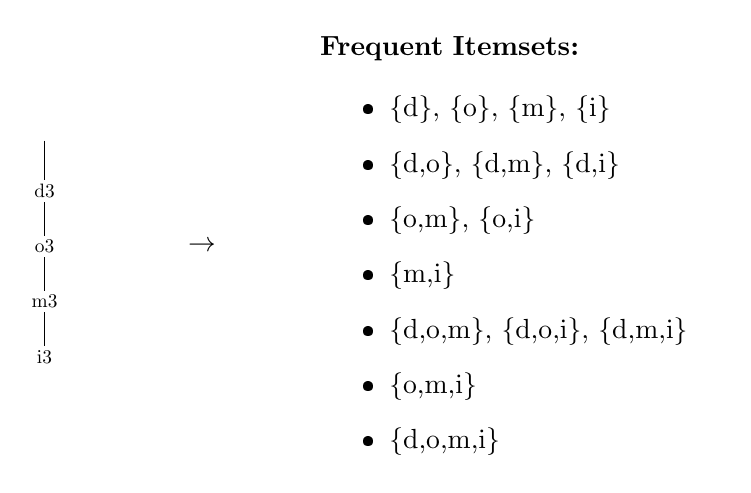
\begin{tikzpicture}
					      % Single branch FP-tree
					      \node[inner sep=0.05cm] at (0,0) (root) {\scalebox{0.7}{\fptreerootnode}};
					      \node[inner sep=0.05cm] at (0,-0.7) (d) {\scalebox{0.7}{\fptreenode{d}{3}}};
					      \node[inner sep=0.05cm] at (0,-1.4) (o) {\scalebox{0.7}{\fptreenode{o}{3}}};
					      \node[inner sep=0.05cm] at (0,-2.1) (m) {\scalebox{0.7}{\fptreenode{m}{3}}};
					      \node[inner sep=0.05cm] at (0,-2.8) (i) {\scalebox{0.7}{\fptreenode{i}{3}}};
					      \draw (root) -- (d) -- (o) -- (m) -- (i);

					      % Arrow
					      \node at (2,-1.4) (arrow) {$\rightarrow$};

					      % Frequent itemsets
					      \node[text width=5cm] at (6,-1.4) (frequent-itemsets) {
						      \textbf{Frequent Itemsets:} \\
						      \begin{itemize}
							      \item \{d\}, \{o\}, \{m\}, \{i\}
							      \item \{d,o\}, \{d,m\}, \{d,i\}
							      \item \{o,m\}, \{o,i\}
							      \item \{m,i\}
							      \item \{d,o,m\}, \{d,o,i\}, \{d,m,i\}
							      \item \{o,m,i\}
							      \item \{d,o,m,i\}
						      \end{itemize}
					      };


				      \end{tikzpicture}
			      }
		      \end{center}
	\end{itemize}
\end{frame}

\begin{frame}{FP-growth - Special Case(s) (II)}
	\begin{itemize}
		\item \textbf{Special Case:} A single prefix path in a FP-tree
		      \begin{itemize}
			      \item Reduction of the single prefix path into one node.
			      \item Concatenation of the mining results of the two parts.
			      \item Both parts can be mined in parallel.
		      \end{itemize}
	\end{itemize}

	\vspace*{0.5cm}

	\begin{center}
		\scalebox{0.7}{
			\begin{tikzpicture}
				\node[inner sep=0.05cm] at (0,0) (0) {\scalebox{0.7}{\fptreerootnode}};
				\node[inner sep=0.05cm] at (0,-0.7) (a1n1) {\scalebox{0.7}{\fptreenode{a\textsubscript{1}}{n\textsubscript{1}}}};
				\node[inner sep=0.05cm] at (0,-1.4) (a2n2) {\scalebox{0.7}{\fptreenode{a\textsubscript{2}}{n\textsubscript{2}}}};
				\node[inner sep=0.05cm] at (0,-2.1) (a3n3) {\scalebox{0.7}{\fptreenode{a\textsubscript{3}}{n\textsubscript{3}}}};
				\node[inner sep=0.05cm] at (-0.7,-2.8) (b1m1) {\scalebox{0.7}{\fptreenode{b\textsubscript{1}}{m\textsubscript{1}}}};
				\node[inner sep=0.05cm] at (0.7,-2.8) (c1k1) {\scalebox{0.7}{\fptreenode{c\textsubscript{1}}{k\textsubscript{1}}}};
				\node[inner sep=0.05cm] at (0,-3.5) (c2k2) {\scalebox{0.7}{\fptreenode{c\textsubscript{2}}{k\textsubscript{2}}}};
				\node[inner sep=0.05cm] at (1.4,-3.5) (c3k3) {\scalebox{0.7}{\fptreenode{c\textsubscript{3}}{k\textsubscript{3}}}};
				\draw (0)--(a1n1)--(a2n2)--(a3n3)--(b1m1);
				\draw (a3n3)--(c1k1);
				\draw (c1k1)--(c2k2);
				\draw (c1k1)--(c3k3);
				\node at (2.1,-2.1) (join) {$\rightarrow$};
				\node[inner sep=0.05cm] at (3.5,-2.1) (r1) {\scalebox{0.7}{\fptreeuniquenode{r\textsubscript{1}}}};
				\node at (4.25,-2.1) (r1equals) {$=$};
				\node[inner sep=0.05cm] at (5,0) (20) {\scalebox{0.7}{\fptreerootnode}};
				\node[inner sep=0.05cm] at (5,-0.7) (2a1n1) {\scalebox{0.7}{\fptreenode{a\textsubscript{1}}{n\textsubscript{1}}}};
				\node[inner sep=0.05cm] at (5,-1.4) (2a2n2) {\scalebox{0.7}{\fptreenode{a\textsubscript{2}}{n\textsubscript{2}}}};
				\node[inner sep=0.05cm] at (5,-2.1) (2a3n3) {\scalebox{0.7}{\fptreenode{a\textsubscript{3}}{n\textsubscript{3}}}};
				\draw (20)--(2a1n1)--(2a2n2)--(2a3n3);
				\node at (7,-2.1) (r1) {$\oplus$};
				\node[inner sep=0.05cm] at (8.4,-2.1) (30) {\scalebox{0.7}{\fptreeuniquenode{r\textsubscript{1}}}};
				\node[inner sep=0.05cm] at (8.1,-2.8) (b1m1) {\scalebox{0.7}{\fptreenode{b\textsubscript{1}}{m\textsubscript{1}}}};
				\node[inner sep=0.05cm] at (9.5,-2.8) (c1k1) {\scalebox{0.7}{\fptreenode{c\textsubscript{1}}{k\textsubscript{1}}}};
				\node[inner sep=0.05cm] at (8.4,-3.5) (c2k2) {\scalebox{0.7}{\fptreenode{c\textsubscript{2}}{k\textsubscript{2}}}};
				\node[inner sep=0.05cm] at (9.9,-3.5) (c3k3) {\scalebox{0.7}{\fptreenode{c\textsubscript{3}}{k\textsubscript{3}}}};
				\draw (30)--(c1k1)--(c3k3);
				\draw (30)--(b1m1);
				\draw (c1k1)--(c2k2);
			\end{tikzpicture}
		}
	\end{center}
\end{frame}

\begin{frame}{Advantages of the FP-growth Approach}
	\begin{itemize}
		\item Can be \textbf{parallelized}:
		      \begin{itemize}
			      \item Different conditional pattern bases can be mined in parallel.
		      \end{itemize}
		\item \textbf{No candidate generation} \\ \hspace*{1cm} $\Rightarrow$ No candidate test required.
		\item Compressed database: FP-tree structure.
		\item Only \textbf{two} scans of the database.
	\end{itemize}
\end{frame}

\subsection{Other Approaches}

\begin{frame}{ECLAT: Mining by Exploring Vertical Data Format}
	\begin{itemize}
		\item \textbf{Vertical format: $t(AB) = \{T_{11},T_{25},\ldots\}$}
		      \begin{itemize}
			      \item Tid-list: list of transaction ids containing an itemset.
		      \end{itemize}
		\item \textbf{Deriving frequent itemsets based on vertical
			      intersections.}
		      \begin{itemize}
			      \item $t(X) = t(Y): \qquad$ \hphantom{.} $X$ and $Y$ always happen
			            together.
			      \item $t(X) \implies t(Y):\quad $ transaction having $X$ always has
			            $Y$.
		      \end{itemize}
		\item \textbf{Using diffset to accelerate mining.}
		      \begin{itemize}
			      \item Only keep track of differences of tids.
			      \item $t(X) = \{T_1,T_2,T_3\}$, $t(XY) = \{T_1,T_3\}$.
			      \item Diffset $(XY,X) = \{T_2\}$.
		      \end{itemize}
		\item \textbf{ECLAT} (Zaki et al., KDD'97)
		\item \textbf{Mining closed itemsets using vertical format: CHARM}
		      (Zaki \& Hsiao, SDM'02)
	\end{itemize}
\end{frame}

\begin{frame}{Mining Closed Itemsets: CLOSET (I)}
	\begin{columns}[c]
		\begin{column}{0.6\textwidth}
			\begin{itemize}
				\item \textbf{F-list: list of all frequent items \\ in
					      support-ascending order.}
				      \begin{itemize}
					      \item F-list: d-a-f-e-c.
				      \end{itemize}
				\item \textbf{Divide search space.}
				      \begin{itemize}
					      \item Itemsets having d.
					      \item Itemsets having d but not a, etc.
				      \end{itemize}
				\item \textbf{Find closed itemsets recursively.}
				      \begin{itemize}
					      \item Every transaction having d also has $cfa \implies
						            cfad$ is a closed itemset.
					      \item (Pei, Han \& Mao, DMKD'00)
				      \end{itemize}
			\end{itemize}
		\end{column}
		\begin{column}{0.25\textwidth}
			\begin{tabular}{|c|c|}
				\hline
				TID & Items     \\\hline
				10  & a,c,d,e,f \\\hline
				20  & a,b,e     \\\hline
				30  & c,e,f     \\\hline
				40  & a,c,d,f   \\\hline
				50  & c,e,f     \\\hline
			\end{tabular}
		\end{column}
	\end{columns}
\end{frame}

\begin{frame}{Mining Closed Itemsets: CLOSET (II)}
	\begin{itemize}
		\item \textbf{Itemset merging:.}
		      \begin{itemize}
			      \item If $Y$ appears in each occurrence of $X$, then $Y$ is merged
			            with $X$.
		      \end{itemize}
		\item \textbf{Sub-itemset pruning:}
		      \begin{itemize}
			      \item If $X \subset Y$ and $\text{sup}(X) = \text{sup}(Y),$ $X$ and
			            all of $X$'s\\
			            descendants in the set enumeration tree can be pruned.
		      \end{itemize}
		\item \textbf{Item skipping:}
		      \begin{itemize}
			      \item If a local frequent item has the same support in several
			            header tables at different levels, \\
			            one can prune it from the header table at higher levels.
		      \end{itemize}
		\item \textbf{Efficient subset checking.}
	\end{itemize}
\end{frame}

\begin{frame}{MaxMiner: Mining Max-itemsets}
	\begin{columns}[c]
		\begin{column}{0.6\textwidth}
			\begin{itemize}
				\item \textbf{1st scan: find frequent items.}
				      \begin{itemize}
					      \item A, B, C, D, E
				      \end{itemize}
				\item \textbf{2nd scan: find support for:}
				      \begin{itemize}
					      \item AB, AC, AD, AE, \textbf{ABCDE}
					      \item BC, BD, BE, \textbf{BCDE}
					      \item CD, CE, \textbf{CDE}, DE
				      \end{itemize}
				\item \textbf{Potential max-itemsets: ABCDE, BCDE, CDE.}
				\item \textbf{Since BCDE is a max-itemset, no need to check
					      BCD, BDE, CDE in later scan.} (Bayardo, SIGMOD'98)
			\end{itemize}
		\end{column}
		\begin{column}{0.3\textwidth}
			\begin{tabular}{|c|c|}
				\hline
				TID & Items     \\\hline
				10  & A,B,C,D,E \\\hline
				20  & B,C,D,E   \\\hline
				30  & A,C,D,F   \\\hline
			\end{tabular}
		\end{column}
	\end{columns}
\end{frame}
